\documentclass[10pt,twoside]{article}
\usepackage[utf8]{inputenc}
\usepackage{amsmath}
\usepackage{amsfonts}
\usepackage{amssymb}
\usepackage[spanish,es-noshorthands]{babel}
\usepackage[T1]{fontenc}
\usepackage{lmodern}
\usepackage{graphicx,hyperref}
\usepackage{tikz,pgf}
\usepackage{multicol}
\usepackage{subfig}
\usepackage[papersize={6.5in,8.5in},width=5.5in,height=7in]{geometry}
\usepackage{fancyhdr}
\pagestyle{fancy}
\fancyhead[LE]{
\includegraphics[height=12pt]{Images/logo-colegio.png} Ética $9^{\circ}$}
\fancyhead[RE]{}
\fancyhead[RO]{\textit{Germ\'an Avenda\~no Ram\'irez, Lic. U.D., M.Sc. U.N.}}
\fancyhead[LO]{}

\author{Germ\'an Avenda\~no Ram\'irez, Lic. U.D., M.Sc. U.N.}
\title{\begin{minipage}{.2\textwidth}

\includegraphics[height=1.75cm]{Images/logo-colegio.png}\end{minipage}
\begin{minipage}{.55\textwidth}
\begin{center}
Taller 06, Cultivo de hábitos  \\
Étitica $9^{\circ}$
\end{center}
\end{minipage}\hfill
\begin{minipage}{.2\textwidth}

\includegraphics[height=1.75cm]{Images/logo-sed.png} 
\end{minipage}}
\date{}
\begin{document}
\maketitle
Nombre: \hrulefill Curso: \underline{\hspace*{44pt}} Fecha: \underline{\hspace*{2.5cm}}
\section*{Lo que s\'{e}}
\subsection*{Antes de comenzar}
\begin{enumerate}
\item ¿Recuerdas la fábula de Esopo sobre la liebre y la tortuga?\\
Lee la siguiente versión, compárala con la original y saca tus propias conclusiones. Luego, desarrolla las actividades.
\end{enumerate}
\subsubsection*{La liebre y la tortuga}
“Una tortuga y una liebre siempre discutían sobre quién
era más rápida. Para dirimir el asunto, decidieron correr
una carrera. Acordaron la ruta, las condiciones y empezó
la competencia. La liebre, sabiéndose veloz, arrancó a toda
velocidad y corrió rauda durante algún trecho. Luego pensó
que llevaba buena ventaja y decidió sentarse bajo un árbol
para descansar, recuperar fuerzas y continuar luego.

Pronto se durmió. Entre tanto la tortuga con su paso lento pero
constante y persistente, la alcanzó, la superó y terminó llegando en
primer lugar, declarándose vencedora indiscutible. Pero la versión
no termina allí. La liebre, decepcionada consigo misma por haber
perdido debido a su pereza y descuido, reflexionó sobre el asunto
y reconoció sus errores, prometiéndose que no la vencerían nunca
más. Desafió nuevamente a la tortuga y corrió con tenacidad de
principio a fin, sin dar por sentada su ventaja y esta vez su triunfo fue
evidente. Pero la tortuga no se conformaba; sabía que como estaba
planteada la carrera, no ganaría. Entonces propuso cambiar la ruta a
lo que accedió la liebre. Se inició una nueva competencia con ventaja
evidente de la liebre que corrió diligente hasta encontrar un río y se
paró frente a él porque no sabía nadar. La tortuga llegó a su lado
al rato, entró al agua y nadando atravesó el río, continuó la marcha
dejando atrás a la liebre y finalmente ganó la carrera”.\footnote{\url{www.epconsultores.com}. Adaptación.
}
\begin{center}
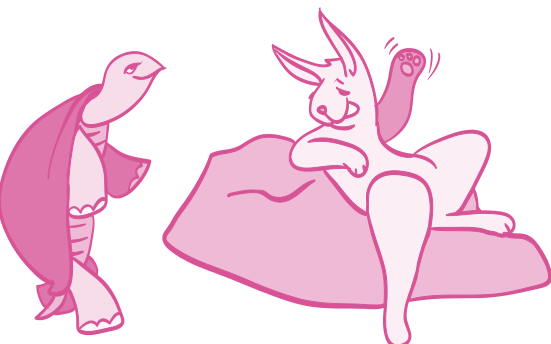
\includegraphics[scale=.65]{Images/liebra_tortuga.png} 
\end{center}
\begin{enumerate}
\item Responde en tu cuaderno: En ambos casos,
¿por qué triunfó la tortuga en la carrera?
\item ¿Qué similitudes y diferencias encuentras
entre tu actitud y la de la tortuga?
\item En equipos de cuatro integrantes, propongan
una o más moralejas asociadas a la fábula
anterior, discútanlas y planteen estrategias
para aplicarlas en el curso.
\end{enumerate}
En el módulo anterior, se definieron los hábitos como las virtudes
que facilitan a las personas actuar correctamente, hacer el bien
y superar las adversidades. Toda acción con consecuencias
favorables amerita repetirse y es allí donde tienen fundamento
los hábitos. Éstos se cultivan cuando las personas reflexionan
continuamente en torno a ellos, no son conformistas y se
muestran dispuestas, disciplinadas, laboriosas y persistentes,
cualidades que a su vez se asocian a numerosas habilidades como
lo demostró la tortuga frente a su adversaria.
\subsection*{Disposici\'{o} y disciplina}
\begin{itemize}
\item La palabra \emph{disposición} hace referencia a la aptitud,
habilidad y condición de ánimo que se tenga para
realizar determinada acción. En tanto que la \emph{disciplina}
es la capacidad de actuar de manera ordenada y
perseverante en el logro de un objetivo. Cumplir
de buena gana con los horarios establecidos o
los compromisos contraídos, por ejemplo, son
hábitos que muestran buena disposición y
disciplina. También lo son mantener una
presentación personal impecable, respetar
la palabra empeñada y asumir con
optimismo y calidad la función social que
nos corresponde como hijos, estudiantes,
ciudadanos y miembros de una comunidad.
En este sentido cada acción corresponde al
principio de que los asuntos del contexto
también corresponden al individuo.
\item Por lo anterior, también es una
expresión de buena disposición
y disciplina, actuar en beneficio
común aunque eso no haga
parte de las tareas habituales
e incluso, aunque no se haya
recibido una orden al respecto.
En eso consiste tomar iniciativas
con función social.
\end{itemize}
\emph{Los buenos hábitos de cada individuo
generan impactos favorables en toda la
comunidad. }
\section*{Ejercito lo aprendido - Evaluaci\'{o}n}
\subsection*{Reflexiona y eval\'{u}a}
 \begin{enumerate}
 \item ¿Cómo calificas tu disposición y disciplina en las
responsabilidades que tienes como miembro de tu familia?
¿En qué actividades podrías mejorar?
\item Haz una lista de cinco actividades escolares. Califica tu
disposición y disciplina en ellas, siendo 1 muy deficiente, con
mucho por mejorar, y 5 un comportamiento excelente.
 \end{enumerate}
 \begin{itemize}
 \item Una persona con buena disposición y disciplina es un
ciudadano organizado, confiable, cumplido, puntual,
que promueve con ello la armonía y el orden, y en
consecuencia, el respeto a sí mismo y hacia los otros.
La disciplina se convierte en un entrenamiento que
corrige, moldea, da fortaleza y perfecciona; contribuye
a formar buenos hábitos y a establecer una serie de
reglas personales que generan compromisos y fortalecen
decisiones. La buena disposición, hace que todos esos
hábitos se fijen en la personalidad. De esa forma no es
necesario que existan agentes externos que controlen
o vigilen la forma como actúan las otras personas pues
sus hábitos son suficientes para controlar sus deseos,
emociones, actitudes y lenguajes. Cuando una persona
logra este nivel de autonomía, demuestra madurez y
verdadera capacidad de reflexión moral.
 \end{itemize}
 \section*{Aprendo algo nuevo}
 \subsection*{Laboriosidad}
 \emph{“El hambre pasa por delante de la casa del hombre laborioso,
pero no se atreve a entrar en ella.”}\footnote{Benjamín Franklin
}
\end{document}
